% latexmal.tex - Mal beregnet for bruk i INF1080
% Time-stamp: <2012-08-27 11:08:39>
%%%%%%%%%%%%%%%%%%%%%%%%%%%%%%%%%%%%%%%%%%%%%%%%%%%%%%%%%%%%%%%%%%%%%%%%%%%
%
% Dette dokumentet har innstillinger som fungerer på Ifi-serverne.
% Du kan lage en pdf-fil av denne filen med:
%  pdflatex latexmal.tex
%
% Et LaTeX-dokument har to deler. Først skriver du inn ting som
% gjelder hele dokumentet, blant annet hvilke pakker du skal bruke.
% Så kommer selve innholdet, mellom \begin{document} og \end{document}
%
% Husk at tegnene: # $ % ^ & _ { } ~ og \ har spesiell betydning.
%
% For mer hjelp og mer info om hvordan du kan stille inn dokumentet
% er disse sidene bra:
% http://www.mn.uio.no/ifi/tjenester/it/hjelp/latex/
% http://en.wikibooks.org/wiki/LaTeX/
%
%%%%%%%%%%%%%%%%%%%%%%%%%%%%%%%%%%%%%%%%%%%%%%%%%%%%%%%%%%%%%%%%%%%%%%

% 1. Hva slags dokument.
\documentclass[12pt,norsk,a4paper]{article}
\usepackage{float}
\usepackage{hyperref}
\usepackage[all]{hypcap}
\usepackage{graphicx}
\graphicspath{ {img/} }


\hypersetup{
    colorlinks,
    citecolor=black,
    filecolor=black,
    linkcolor=black,
    urlcolor=blue
}

\usepackage{apacite}
\usepackage{mathtools}
\usepackage{amsmath}
% For eget tittelblad: legg ,titlepage til rett etter a4paper
% For tosidig: legg til ,twopage


% 3. Norske tegn og norsk utseende

% 3a. Tekstfiler med norske tegn kan lagres i utf-8 eller iso-latin-1
% (iso-8859-1). På Ifi-maskinene er iso-8859-1/15 standard.
\usepackage[utf8]{inputenc} % evt utf8 i stedet for latin1
%\DeclareUnicodeCharacter{030A}{~}

% Please add the following required packages to your document preamble:
\usepackage[table,xcdraw]{xcolor}
% If you use beamer only pass "xcolor=table" option, i.e. \documentclass[xcolor=table]{beamer}
\usepackage{listings}
\usepackage[title]{appendix}
% 2. Om dokumentet - brukes blant annet til tittelen
\title{Numerical analysis - Matteprosjekt}
\author{Sondre Løvhaug, Dan Rasmussen,\\
	Eiric Halland Wærness, Håvard Granaune Matberg
}
\date{\today}


% 3b. For norsk orddeling og dato
\usepackage[norsk]{babel}
\usepackage[norsk]{isodate}

% 3c. For norske tegn
\usepackage[T1]{fontenc}

% 3d. For parallelle avsnitt (fint i INF1080, men ikke så fint i vanlige artikler)
\usepackage{parskip}

% 3e. For å formattere URL-er.
%\usepackage{url}

% 4. Skrifttype og symboler
\usepackage[small,euler-digits]{eulervm}
%\usepackage[bitstream-charter]{mathdesign}
\usepackage{color}

% 5. For litt mindre marger enn standard i LaTeX
\usepackage{a4wide}
\usepackage[top=2cm, margin=2.5cm]{geometry}

% 6. Figurer og bilder

% 6a. For å bryte tekst rundt en figur
%\usepackage{wrapfig}

% 6b. For bilder - med denne pakken kan du legge inn bilder og
% illustrasjoner slik:
%                  \includegraphics[width=.5\textwidth]{bilde.pdf}
\usepackage{graphicx}
\graphicspath{ {img/} }

% 7. For grafer og slikt
%\usepackage{tikz}
%\usetikzlibrary{trees}
% Det fins mange tikz-bibliotek, det er nesten ingen grenser for hva
% du kan lage med dette. Se http://www.texample.net/tikz/

% 8. Egendefinerte kommandoer kan du legge inn slik:
\newcommand{\tuple}[1]{\ensuremath{\langle #1\rangle}}
\newcommand{\set}[1]{\ensuremath{\{#1\}}}
\newcommand{\imp}{\ensuremath{\rightarrow}}
\newcommand{\M}{\ensuremath{\mathcal{M}}}
\newcommand{\AF}{edge from parent[draw=none]}
\newcommand{\NODE}[1]{\{node \{\ensuremath{#1}\}\}}
% http://en.wikibooks.org/wiki/LaTeX/Customizing_LaTeX#New_commands
\usepackage{textcomp}

% 9. Pakke for å formatere Matlab-dokumneter:

\usepackage[]{mcode}


%%%%%%%%%%%%%%%%%%%%%%%%%%%%%%%%%%%%%%%%%%%%%%%%%%%%%%%%%%%%%%%%%%%%%%%%%%%
% Selve innholdet:
\begin{document}

% a. Lager en tittel på dokumentet.
\maketitle
% a. For å få bokstavnummerering på 'subsection's
%\renewcommand{\thesubsection}{(\alph{subsection})}
%\vspace{20mm}

\newpage
\textbf{Revisjonshistorie} \\
\begin{tabular}{|l|l|l|l|}
    \hline
    \textbf{Dato} & \textbf{Versjon} & \textbf{Beskrivelse} & \textbf{Forfatter} \\
    \hline
    26 Januar 2016 & 0.1 & Første versjon & ESN \\
    \hline
\end{tabular}
\newpage
\tableofcontents
%\listoffigures
%\listoftables
\newpage

\section{Innledning}
Gruppe 11 ble sammensatt av at vår faglærer teamet sammen Sondre Løvhaug og Dan Rasmussen sammen med Håvard Matberg og Eric Wærness. Vi har ikke jobbet sammen på tidligere prosjekt, men det virker som gruppa ble en fin match. Etter første møte med faglærer gikk vi løst på oppgavesettet. Ved første øyekast kunne det virke noe utfordrende, men med den ustoppelige kraften fra samarbeid fikk vi raskt kommet i gang med, og løst, første oppgave.
\newpage
\section{Teori}

\subsection{Eurler-Bernoulli}
Flere av oppgavene i denne rapporten omhandler Euler-Bernoulli-bjelken. I følge Wikipedia er dette en grunnleggende metode for å regne ut hvor mye en bjelke av et gitt materiale bøyer seg under press. Metoden er oppkalt etter Jacob Bernoulli som gjorde de største oppdagelsene, det var derimot ikke før rundt 1750 at Leonhard Euler og Daniel Bernoulli kom opp med en komplett teori. Metoden ble ikke brukt i praksis på noen større prosjekter før byggingen av Eiffeltårnet i 1889, men har siden blitt en hjørnestein innen ingeniørkunsten.\footnote{\url{https://en.wikipedia.org/wiki/Euler-Bernoulli_beam_theory}, (14.04.2016)} Euler-Bernoulli-likningen er som følger:
\begin{quote}
\begin{equation}
EIy''''=f(x)
\end{equation}
\end{quote}
Den vertikale forskyvningen av en $L$ meter lang bjelke, , oppfyller likningen når $0\leq x\leq L$. Likningen inneholder noen konstanter; $E$ er en materialkonstant kalt Youngmodulusen. $I$ er et arealmoment til bjelkens tverrsnitt normalt på lengderetningen. $I$ er konstant langs hele bjelken. Høyresiden av likningen, $f(x)$, er en kraft som virker på bjelken per lengde-enhet målt i Newton per meter. Kraften inkluderer vekten til bjelken. Dette har vi fra læreboken.\footnote{Sauer, Timothy, (2012) Numerical Analysis second edition, side 102-.}

Hvorfor kan dette brukes på stupebrett?
Legge til ekstra kraft for haug og person.

\subsection{Numerisk kontra Korrekt}

\subsection{Taylors Teorem}
Taylors Teorem er en måte å estimere en gitt funksjon på ved hjelp av polynomer. Man kan se på Taylors formel som en generalisering av "Mean Value Theorem", som sier at dersom funksjonen f er kontinuerlig i et lukket intervall [a,b] og f er deriverbar i det åpne intervallet (a,b), et punkt c, a < c < b eksisterer slik at :
\begin{quote}
\begin{equation}
f'(c) = \frac{f(b) - f(a)}{b-a}
\end{equation}
\end{quote}
Mer bestemt, la f være en funksjon slik at f og dens første n-deriverte er kontinuerlig i [a,b]. Videre, la $f^{(n+1)}(x)$ eksistere for alle x i (a,b). Da eksisterer det et tall c i (a,b) slik at:
\begin{quote}
\begin{equation}
f(b) = f(a) + (b-a) \frac{f'(a)}{1!} + (b-a)^2 \frac{f''(a)}{2!} + .... + (b-a)^n \frac{f^{(n)}}{n!} + (b-a)^{(n+1)} \frac{f^{(n+1} (c)}{(n+1)!}
\end{equation}
\end{quote}
Formelen sier også at dersom b < a, så vil [a,b] og (a,b) blir byttet ut med [b,a] og (b,a) henholdsvis. Man kan også se at dersom vi bytter ut b med x, står vi igjen med Taylor's formelen. \\
En annen måte å skrive Taylor's formelen på er
\begin{quote}
\begin{equation}
\sum_{i=0}^n (x-a)î \frac{f''(a)}{i!} + (x-a)^{n+1} \frac{f^{(n+1)} (c) }{(n+1)!}
\end{equation}
\end{quote}
som også er kjent som n-te grad Taylor polynom (eller Taylor serie) med feil ledd.\\
For å visualisere dette kan vi ta for oss funksjonen $f(x) = sin(x)$. Ved å regne ut flere ledd i Taylor-rekken vil vi kunne skape en tilnærming av funksjonen. Desto flere ledd, desto mer nøyaktig tilnærming:

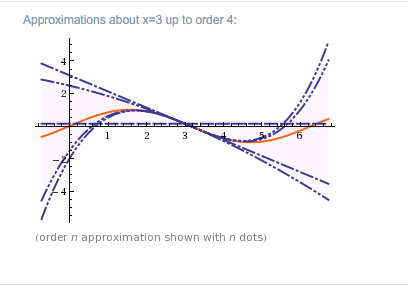
\includegraphics[width=\textwidth]{taylor_sinx}
Grafen er en taylors-rekke av f(x) = sin(x), der x=3. Studerer man de blå striplette linjene ser vi at de inneholder ulikt antall prikker. 1 prikk tilsvarer første deriverte, 2prikker tilsvarer andre deriverte osv. Ut i fra grafen ser man at dersom man har et høyere derivasjonsledd vil den blå linjen følge funksjonen mer og mer, og vi får en mer nøyaktig tilnærming av funksjonen. 


\subsection{Kondisjonstall}

\subsection{Feil}
Forover og bakoverfeil.

\subsection{MATLAB}

\subsection{Teori tilknyttet oppgaver}
\subsubsection{Oppgave 3}
Møtte på et problem tilknyttet oppgave 3 hvor vi fikk positive verdier for y. Etter lang leting viste det seg at i vår lagA- metode så hadde vi klart å skreve -157/17 kontra -156/17 som det egentlig skulle være. Var spennende å se at en så liten feil kunne resultere til så forskjellige verdier. 

\newpage
\section{Utregning}

\subsection{Oppgave 1}
\subsubsection{Oppgave 5.1.21}
Prove the second-order formula for the fourth derivative
\begin{quote}
\begin{equation}\label{eq:oppgave1}
f^{(4)} (x) = \frac{f(x-2h) - 4f(x-h) + 6f(x) - 4f(x+h) + f(x+2h)}{h^4} + O(h^2)
\end{equation}
\end{quote}
Ifølge Taylor's teorem, dersom f er fem ganger kontinuerlig deriverbar, 
kan vi bruke f(x + h) og f(x -h)
\begin{quote}
\begin{equation} \label{eq:f(x+h)}
f(x+h) = f(x) + hf'(x) + \frac{h^2}{2} f''(x) + \frac{h^3}{6} f'''(x) + \frac{h^4}{24} f^4 (x) + \frac{h^5}{120} f^5 (x) + O(h^6)
\end{equation}
\end{quote}
\begin{quote}
\begin{equation} \label{eq:f(x-h)}
f(x-h) = f(x) - hf'(x) + \frac{h^2}{2} f''(x) - \frac{h^3}{6} f'''(x) + \frac{h^4}{24} f^4 (x) - \frac{h^5}{120} f^5 (x) + O(h^6)
\end{equation}
\end{quote}
Legger så sammen f(x+h) + f(x-h) for å eliminere odde-talls deriverte:

\begin{multline} \label{eq:f(x+h)+f(x-h)}
f(x+h) + f(x-h) = \\f(x) + hf'(x) + \frac{h^2}{2} f''(x) + \frac{h^3}{6} f'''(x) + \frac{h^4}{24} f^4 (x) + \frac{h^5}{120} f^5 (x) + O(h^6) +\\
 f(x) - hf'(x) + x\frac{h^2}{2} f''(x) - \frac{h^3}{6} f'''(x) + \frac{h^4}{24} f^4 (x) - \frac{h^5}{120} f^5 (x) + O(h^6) \\ = 2f(x) + h^2 f''(x) + \frac{h^4}{12} f^{(4)} (x) + O (h^6)
\end{multline}
I følge Taylor's teorem, dersom f er fem ganger kontinuerlig deriverbar, kan vi bruke f(x+2h) og f(x-2h). \\
Legger så sammen f(x+2h) + f(x-2h) for å eliminere oddetalls-deriverte. \\
Siden vi allerede har regnet ut f(x+h) + f(x-h), setter vi inn for f(x+2h) og f(x-2h) og får:
\begin{equation} \label{eq:f(x+2h)+f(x-2h)}
f(x+2h) + f(x-2h) = 2f(x) + 2h^2 f(x) + \frac{4h^4}{3} f^4 (x) + O (h^6)
\end{equation}
For å få den fjerde-deriverte aleine, må vi eliminere den andre-deriverte. Dette gjøres ved å gange inn 4 i den første likningen (\ref{eq:f(x+h)+f(x-h)}) og trekker fra likning (\ref{eq:f(x+2h)+f(x-2h)}): 

\begin{multline*}
4 * (f(x+h) + f(x-h)) = 8f(x) + 4h^2 f''(x) + \frac{4h^4}{12} f^4 + 4O(h^6) \\
\Downarrow
\\
4f(x+h) + 4f(x-h) - (f(x+2h) + f(x-2h)) = \\ 
8f(x) + 4h^2 f''(x) + \frac{4h^4}{12} f^4 (x) + 4O(h^6) - \\
2f(x) + 2h^2 f(x) + \frac{4h^4}{3} f^4 (x) + O (h^6) \\
= 6f(x) - h^4 f^4 (x) + 3O (h^6)
\end{multline*}
Snur litt om på likningen og får at:
\begin{multline}
h^4 f^4 = -4f(x+h) - 4f(x-h) + f(x-2h) + f(x-2h) + 6f(x) + 3O(h^6)\\
\Rightarrow f^4 (x) = \frac{f(x-2h) - 4f(x-h) + 6f(x) - 4f(x+h) + f(x+2h)}{h^4} + O(h^2)
\end{multline}


\subsubsection{Oppgave 5.1.22a}
Prove that if f(x) = f'(x) = 0, then
\begin{quote}
\begin{equation}\label{eq:oppgave2}
f^{(4)} (x + h) - \frac{16f(x + h) - 9f(x + 2h) + \frac{8}{3}f(x + 3h) - \frac{1}{4}f(x + 4h)}{h^4} = O(h^2)
\end{equation}
\end{quote}
Starter med å bevise at dersom f(x) = f'(x) = 0, så er
\begin{quote}
\begin{equation}
f(x + h) - 10f(x+h) + 5f(x + 2h) - \frac{5}{3}f(x + 3h) - \frac{1}{4}(x+4h) = O(h^6)
\end{equation}
\end{quote}
Fra oppgave 1, 5.1.21 har vi (\ref{eq:oppgave1}), vi begynner med å skrive denne om til f(x+h) og får:
\begin{quote}
\begin{equation}\label{eq:f^4(x+h)}
f^{(4)}(x+h) = \frac{-4f(x) + f(x-h) + 6f(x+h) - 4f(x+2h) f(x+3h}{h^4} + O(h^2)
\end{equation}
\end{quote}

Nå har vi en likning for $ f^{(4)} (x+h)$ og kan sette denne inn i (\ref{eq:oppgave2})


\begin{multline*}
\frac{-4f(x) + f(x-h) + 6f(x+h) - 4f(x+2h) + f(x+3h)}{h^4} + O(h^2)\\
-
\\
\frac{16f(x+h) - 4f(x+2h) + \frac{8}{3}f(x+3h) - \frac{1}{4}f(x+4h)}{h^4}  = O(h^2)
\\
\Downarrow
\\
\frac{-4f(x)+f(x-h)-10f(x+h)+5f(x+2h)-\frac{5}{3}f(x+3h)+\frac{1}{4}f(x+4h}{h^4} + O(h^2) = O(h^2)
\end{multline*}
Fra oppgaveteksten har vi oppgitt at:
\begin{equation*}
f(x-h)-10f(x+h)+5f(x+2h)-\frac{5}{3}f(x+3h)+\frac{1}{4}f(x+4h) = O(h^6)
\end{equation*}

Vi setter dette inn i likninger vår og får:

\begin{equation*}
\frac{-4f(x) + O(h^6)}{h^4} + O(h^2) = O(h^2)
\end{equation*}

Siden f(x) = f'(x) = 0 ender vi med:


\begin{equation*}
\frac{-0+ O(h^6)}{h^4} + O(h^2) = O(h^2)
\end{equation*}
\begin{equation*}
\Downarrow
\end{equation*}
\begin{equation*}
O(h^2) + O(h^2) = O(h^2)
\end{equation*}

\subsection{Oppgave 2}

lagA.m
\begin{lstlisting}
function A = lagA(n)

e = ones(n,1);
A = spdiags(e*[1 -4 6 -4 1],-2:2,n,n);

A(1,1:4) = [16 -9 8/3 -1/4];
A(n-1,n-3:n) = [16/17 -60/17 72/17 -28/17];
A(n,n-3:n)= [-12/17 96/17 -156/17 72/17];

end
\end{lstlisting}

Scriptet for å kjøre koden:
\begin{lstlisting}
disp('Oppave 2')

A = lagA(10);
full(A)
\end{lstlisting}

\subsection{Oppgave 3}

ebbeam.m
\\
Kan sende med A i fra forrige oppgave, men velger å lage A på nytt slik at dette kan kjøres som et eget skript.
\begin{lstlisting}
% Input:
% E = young's modulus for a meterial
% L = length
% d = diameter
% g = gravity
% w = width
% D = density
function y = ebbeam(E,L,d,D,w,n)

I = w*d^3/12;
h = L/n;
g = 9.81;
b = repmat(-D*w*d*g , n,1) * h^4/(E*I);

A = lagA(n);

y = A\b;
end
\end{lstlisting}
Scriptet for å kjøre koden:
\begin{lstlisting}
disp('Oppgave 3')
format long;
E = 1.3e10;
D = 480;
w = 0.3;
L = 2;
d = 0.03;
n = 10;

disp('Numerisk losning')
y = ebbeam(E,L,d,D,w,n)
\end{lstlisting}

\subsection{Oppgave 4}
\subsubsection{Oppgave 4a}
Vi har at Euler-Bernouillilikningen,
\begin{quote}
\begin{equation}
EIy'''' = f(x)
\end{equation}
\end{quote}
er oppfylt av y(x), som er den vertikale forskyvningen av en L meter lang bjelke. Den korrekte løsningen av likningen med konstanten f(x) = f er;
\begin{quote}
\begin{equation}
y(x)=(f/24EI)*x^2*(x^2-4Lx+6L^2)
\end{equation}
\end{quote}
Skal nå vise at y(x) er den korrekte løsningen ved å derivere den fire ganger og sette inn i Euler-Bernouillilikningen. Begynner med å finne den deriverte med hensyn på x. Vi behandler f/EI og L som konstanter.

Begynner med å finne den deriverte:
\begin{quote}
\begin{equation*}
y=(f/24EI)(x^4-4Lx^3+6L^2x^2)=
\end{equation*}
\begin{equation*}
y'=\frac{d}{dx}[(f/24EI)]\frac{d}{dx}[x^4-4Lx^3+6L^2x^2]=
\end{equation*}
\begin{equation*}
y'=(f/24EI)(4x^3-12Lx^2+12L^2x)=
\end{equation*}
\end{quote}
Her er den derivert en gang, fortsetter med å finne den andrederiverte:
\begin{quote}
\begin{equation*}
y''=\frac{d}{dx}[(f/24EI)]\frac{d}{dx}[4x^3-12Lx^2+12L^2x]=
\end{equation*}
\begin{equation*}
y''=(f/24EI)(12x^2-24Lx+12L^2)=
\end{equation*}
\end{quote}
Her har vi funnet den andrederiverte, fortsetter med å finne den tredjederiverte;
\begin{quote}
\begin{equation*}
y'''=\frac{d}{dx}[(f/24EI)]\frac{d}{dx}[12x^2-24Lx+12L^2]=
\end{equation*}
\begin{equation*}
y'''=(f/24EI)(24x-24L+0)=
\end{equation*}
\end{quote}
Her har vi funnet den tredjederiverte, fortsetter med å finne den fjerdederiverte;
\begin{quote}
\begin{equation*}
y''''=\frac{d}{dx}[(f/24EI)]\frac{d}{dx}[24x-24L]=
\end{equation*}
\begin{equation*}
y''''=(f/24EI)(24)=
\end{equation*}
\begin{equation*}
y''''=\frac{24f}{24EI}
\end{equation*}
\begin{equation*}
y''''=\frac{f}{EI}
\end{equation*}
\end{quote}
Vi har nå funnet den fjerdederiverte til y(x). Vi kan nå sette inn i Euler-Bernouillilikningen;
\begin{quote}
\begin{equation*}
(1) y'''' = \frac{f(x)}{EI}
\end{equation*}
\begin{equation*}
(2) EIy'''' = f(x)
\end{equation*}
\end{quote}
Setter likning (1) inn i likning (2)
\begin{quote}
\begin{equation*}
EI*\frac{f(x)}{EI} = f(x)
\end{equation*}
\begin{equation*}
f(x) = f(x)
\end{equation*}
\end{quote}
Her har vi vist at y(x) oppfyller likningen ved å derivere fire ganger.

\subsubsection{Oppgave 4b}
Skal vise at for den korrekte løsningen er $y^{(6)}$(c) = 0. Vi vet fra oppgave 4a at den 4. deriverte av den korrekte løsningen er:
\begin{equation*}
y^{(4)}(x) = \frac{f}{EI}
\end{equation*}
Vi kan derfra visa at den 6. deriverte er 0.
\begin{equation}
f^{(5)}(x) = \frac{d}{dx}[\frac{f}{EI}] = 0
\end{equation}
Deriverer m.h.p x og $\frac{f}{EI}$ er en konstant.
\begin{equation}
y^{(6)}(x) = \frac{d}{dx}[0] = 0
\end{equation}
Slik har vi vist at $y^{(6)}(c) = 0$.

\subsection{Oppgave 6}
\subsubsection{Oppgave 6a}
Vi legger til en funksjon i Euler-likningen
\begin{quote}
$s(x) = -pgsin\frac{\pi}{L} x $
\end{quote} 
til kraftdelen til f(x)
\begin{quote}
$EIy^{(4)} = f(x) + s(x)$
\end{quote}
Skal bevise at
\begin{quote}
\begin{equation}
y(x) = \frac{f}{24EI} x^2 (x^2 - 4Lx + 6L^2) - \frac{gpL}{EI\pi} (\frac{L^3}{\pi^3} sin\frac{\pi}{L}x - \frac{x^3}{6} + \frac{Lx^2}{2} - \frac{L^2 x}{\pi^2})
\end{equation}
\end{quote}
tilfredstiller Euler-Bernoullie likningen og randbetingelsene for en bjelke som er fast i den ene enden og fri i den andre\\
$y(0) = y'(0) = y''(L) = y'''(L) = 0$ \\
\\
1. Starter med å bevise at y(0)= 0
\begin{quote}
\begin{multline*}
y(0) = \frac{f}{24EI} 0^2 (0^2 - 4L0 + 6L^2) - \frac{gpL}{EI\pi} (\frac{L^3}{\pi^3} sin\frac{\pi}{L}x - \frac{0^3}{6} + \frac{L0^2}{2} - \frac{L^2 0}{\pi^2}) \\
y(0) = 0 - \frac{gpL}{EI\pi} (\frac{L^3}{\pi^3} sin (0) - 0 + 0 - 0 ) \\
y(0) = 0
\end{multline*}
\end{quote}
Første kriterie er oppfylt.
\\
2. Skal nå bevise kriterie 2, at y'(0) = 0, starter med å finne den deriverte.
\begin{quote}
\begin{multline}
y'(x) = \frac{d}{dx} [\frac{fx^2(x^2-4Lx+6L^2)}{24EI} - \frac{gpL}{EI\pi} (\frac{L^3}{\pi^3} sin \frac{\pi}{L}x - \frac{x^3}{6} + \frac{Lx^2}{2} - \frac{L^2x}{\pi^2})]
\end{multline}
\end{quote}

\begin{quote}
\begin{multline*}
y'(x) = \frac{fx(x^2-3Lx+3L^2)}{6EI} - \frac{gpL}{EI\pi}*\frac{d}{dx} (\frac{L^3}{\pi^3} sin \frac{\pi}{L}x - \frac{x^3}{6} + \frac{Lx^2}{2} - \frac{L^2x}{\pi^2})
\end{multline*}
\end{quote}

\begin{quote}
\begin{multline*}
y'(x) = \frac{fx(x^2-3Lx+3L^2)}{6EI} - \frac{gpL}{EI\pi} (\frac{L^2}{\pi^2} cos(\frac{\pi}{L}x) - \frac{x^2}{2} + Lx - \frac{L^2}{\pi^2})
\end{multline*}
\end{quote}
Sjekker om y'(0) = 0
\begin{quote}
\begin{multline*}
y'(0) = \frac{f0(0^2-3L0+3L^2)}{6EI} - \frac{gpL}{EI\pi} (\frac{L^2}{\pi^2} cos(\frac{\pi}{L}0) - \frac{0^2}{2} + L0 - \frac{L^2}{\pi^2})
\end{multline*}
\end{quote}

\begin{quote}
\begin{equation*}
y'(0) = 0 - \frac{gpL}{EI\pi} (\frac{L^2}{\pi^2} * 1 -\frac{L^2}{\pi^2}) \\
\end{equation*}
\end{quote}

\begin{quote}
\begin{equation*}
y'(0) = 0 - \frac{gpL}{EI\pi} (0) = 0
\end{equation*}
\end{quote}
Andre kriteriet er oppfylt.
\\
3. Skal nå bevise kriteriet 3, y''(L) = 0. Starter med å finne den andre deriverte.
\begin{quote}
\begin{multline*}
y'(x) = \frac{fx(x^2-3Lx+3L^2)}{6EI} - \frac{gpL}{EI\pi} (\frac{L^2}{\pi^2} cos(\frac{\pi}{L}x) - \frac{x^2}{2} + Lx - \frac{L^2}{\pi^2})
\end{multline*}
\end{quote}
Fra oppgave 4a, vet vi at
\begin{quote}
\begin{multline*}
y''(x) = \frac{f(x-L)^2}{2EI} - \frac{gpL}{EI\pi} \frac{d}{dx}(\frac{L^2}{\pi^2} cos(\frac{\pi}{L}x) - \frac{x^2}{2} + Lx - \frac{L^2}{\pi^2})
\end{multline*}
\end{quote}

\begin{quote}
\begin{multline}
y''(x) = \frac{f(x-L)^2}{2EI} - \frac{gpL}{EI\pi}* [\frac{L}{\pi} (-sin(\frac{\pi}{L}x)) - x + L]
\end{multline}
\end{quote}
Sjekker nå om y''(L)=0
\begin{quote}
\begin{multline}
y''(L) = \frac{f(L-L)^2}{2EI} - \frac{gpL}{EI\pi}* [\frac{L}{\pi} (-sin(\frac{\pi}{L}L)) - L + L]
\end{multline}
\end{quote}

\begin{quote}
\begin{equation*}
y''(L) = 0 - \frac{gpL}{EI\pi}* [\frac{L}{\pi} (-sin(\pi)) ]
\end{equation*}
\end{quote}

\begin{quote}
\begin{equation*}
y''(L) = 0 - \frac{gpL}{EI\pi}* [\frac{L}{\pi} (0) ]
\end{equation*}
\end{quote}

\begin{quote}
\begin{equation*}
y''(L) = 0 - 0 = 0
\end{equation*}
\end{quote}
Tredje kriteriet stemmer da y''(L) = 0.
4. Skal nå bevise at fjerde kriteriet, y'''(L) = 0, og starter med å finne den tredje deriverte
\begin{quote}
\begin{multline*}
y''(x) = \frac{f(x-L)^2}{2EI} - \frac{gpL}{EI\pi}(\frac{L^2}{\pi^2} cos(\frac{\pi}{L}x) - \frac{x^2}{2} + Lx - \frac{L^2}{\pi^2})
\end{multline*}
\end{quote}

\begin{quote}
\begin{multline*}
y'''(x) = \frac{f(x-L)^2}{2EI} - \frac{gpL}{EI\pi} \frac{d}{dx}(\frac{L^2}{\pi^2} cos(\frac{\pi}{L}x) - \frac{x^2}{2} + Lx - \frac{L^2}{\pi^2})
\end{multline*}
\end{quote}

\begin{quote}
\begin{equation}
y'''(x) = \frac{f(x-L)}{EI} - \frac{gpL}{EI\pi} (-cos(\frac{\pi}{L}x) - 1)
\end{equation}
\end{quote}
Sjekker så tredje kriteriet, y'''(L) = 0
\begin{quote}
\begin{equation*}
y'''(L) = \frac{f(L-L)}{EI} - \frac{gpL}{EI\pi} (-cos(\frac{\pi}{L}L) - 1)
\end{equation*}
\end{quote}

\begin{quote}
\begin{equation*}
y'''(L) = 0 - \frac{gpL}{EI\pi} (1 - 1)
\end{equation*}
\end{quote}

\begin{quote}
\begin{equation*}
y'''(L) = 0 - \frac{gpL}{EI\pi} 0 = 0
\end{equation*}
\end{quote}
Fjerde kriteriet stemmer fordi y'''(L) = 0.

\newpage
\section{Vedlegg}

\subsection{Oppgave 1}
\subsubsection{Oppgave 5.1.21}
Prove the second-order formula for the fourth derivative
\begin{quote}
\begin{equation}\label{eq:oppgave1}
f^{(4)} (x) = \frac{f(x-2h) - 4f(x-h) + 6f(x) - 4f(x+h) + f(x+2h)}{h^4} + O(h^2)
\end{equation}
\end{quote}
Ifølge Taylor's teorem, dersom f er fem ganger kontinuerlig deriverbar, 
kan vi bruke f(x + h) og f(x -h)
\begin{quote}
\begin{equation} \label{eq:f(x+h)}
f(x+h) = f(x) + hf'(x) + \frac{h^2}{2} f''(x) + \frac{h^3}{6} f'''(x) + \frac{h^4}{24} f^4 (x) + \frac{h^5}{120} f^5 (x) + O(h^6)
\end{equation}
\end{quote}
\begin{quote}
\begin{equation} \label{eq:f(x-h)}
f(x-h) = f(x) - hf'(x) + \frac{h^2}{2} f''(x) - \frac{h^3}{6} f'''(x) + \frac{h^4}{24} f^4 (x) - \frac{h^5}{120} f^5 (x) + O(h^6)
\end{equation}
\end{quote}
Legger så sammen f(x+h) + f(x-h) for å eliminere odde-talls deriverte:

\begin{multline} \label{eq:f(x+h)+f(x-h)}
f(x+h) + f(x-h) = \\f(x) + hf'(x) + \frac{h^2}{2} f''(x) + \frac{h^3}{6} f'''(x) + \frac{h^4}{24} f^4 (x) + \frac{h^5}{120} f^5 (x) + O(h^6) +\\
 f(x) - hf'(x) + x\frac{h^2}{2} f''(x) - \frac{h^3}{6} f'''(x) + \frac{h^4}{24} f^4 (x) - \frac{h^5}{120} f^5 (x) + O(h^6) \\ = 2f(x) + h^2 f''(x) + \frac{h^4}{12} f^{(4)} (x) + O (h^6)
\end{multline}
I følge Taylor's teorem, dersom f er fem ganger kontinuerlig deriverbar, kan vi bruke f(x+2h) og f(x-2h). \\
Legger så sammen f(x+2h) + f(x-2h) for å eliminere oddetalls-deriverte. \\
Siden vi allerede har regnet ut f(x+h) + f(x-h), setter vi inn for f(x+2h) og f(x-2h) og får:
\begin{equation} \label{eq:f(x+2h)+f(x-2h)}
f(x+2h) + f(x-2h) = 2f(x) + 2h^2 f(x) + \frac{4h^4}{3} f^4 (x) + O (h^6)
\end{equation}
For å få den fjerde-deriverte aleine, må vi eliminere den andre-deriverte. Dette gjøres ved å gange inn 4 i den første likningen (\ref{eq:f(x+h)+f(x-h)}) og trekker fra likning (\ref{eq:f(x+2h)+f(x-2h)}): 

\begin{multline*}
4 * (f(x+h) + f(x-h)) = 8f(x) + 4h^2 f''(x) + \frac{4h^4}{12} f^4 + 4O(h^6) \\
\Downarrow
\\
4f(x+h) + 4f(x-h) - (f(x+2h) + f(x-2h)) = \\ 
8f(x) + 4h^2 f''(x) + \frac{4h^4}{12} f^4 (x) + 4O(h^6) - \\
2f(x) + 2h^2 f(x) + \frac{4h^4}{3} f^4 (x) + O (h^6) \\
= 6f(x) - h^4 f^4 (x) + 3O (h^6)
\end{multline*}
Snur litt om på likningen og får at:
\begin{multline}
h^4 f^4 = -4f(x+h) - 4f(x-h) + f(x-2h) + f(x-2h) + 6f(x) + 3O(h^6)\\
\Rightarrow f^4 (x) = \frac{f(x-2h) - 4f(x-h) + 6f(x) - 4f(x+h) + f(x+2h)}{h^4} + O(h^2)
\end{multline}


\subsubsection{Oppgave 5.1.22a}
Prove that if f(x) = f'(x) = 0, then
\begin{quote}
\begin{equation}\label{eq:oppgave2}
f^{(4)} (x + h) - \frac{16f(x + h) - 9f(x + 2h) + \frac{8}{3}f(x + 3h) - \frac{1}{4}f(x + 4h)}{h^4} = O(h^2)
\end{equation}
\end{quote}
Starter med å bevise at dersom f(x) = f'(x) = 0, så er
\begin{quote}
\begin{equation}
f(x + h) = 10f(x+h) + 5f(x + 2h) - \frac{5}{3}f(x + 3h) - \frac{1}{4}(x+4h) = O(h^6)
\end{equation}
\end{quote}
Fra oppgave 1, 5.1.21 har vi (\ref{eq:oppgave1}), vi begynner med å skrive denne om til f(x+h) og får:
\begin{quote}
\begin{equation}\label{eq:f^4(x+h)}
f^{(4)}(x+h) = \frac{-4f(x) + f(x-h) + 6f(x+h) - 4f(x+2h) f(x+3h}{h^4} + O(h^2)
\end{equation}
\end{quote}

Nå har vi en likning for $ f^{(4)} (x+h)$ og kan sette denne inn i (\ref{eq:oppgave2})


\begin{multline*}
\frac{-4f(x) + f(x-h) + 6f(x+h) - 4f(x+2h) + f(x+3h)}{h^4} + O(h^2)\\
-
\\
\frac{16f(x+h) - 4f(x+2h) + \frac{8}{3}f(x+3h) - \frac{1}{4}f(x+4h)}{h^4}  = O(h^2)
\\
\Downarrow
\\
\frac{-4f(x)+f(x-h)-10f(x+h)+5f(x+2h)-\frac{5}{3}f(x+3h)+\frac{1}{4}f(x+4h}{h^4} + O(h^2) = O(h^2)
\end{multline*}
Fra oppgaveteksten har vi oppgitt at:
\begin{equation*}
f(x-h)-10f(x+h)+5f(x+2h)-\frac{5}{3}f(x+3h)+\frac{1}{4}f(x+4h) = O(h^6)
\end{equation*}

Vi setter dette inn i likninger vår og får:

\begin{equation*}
\frac{-4f(x) + O(h^6)}{h^4} + O(h^2) = O(h^2)
\end{equation*}

Siden f(x) = f'(x) = 0 ender vi med:


\begin{equation*}
\frac{-0+ O(h^6)}{h^4} + O(h^2) = O(h^2)
\end{equation*}
\begin{equation*}
\Downarrow
\end{equation*}
\begin{equation*}
O(h^2) + O(h^2) = O(h^2)
\end{equation*}

\subsection{Oppgave 6}
\subsubsection{Oppgave 6a}
Vi legger til en funksjon i Euler-likningen
\begin{quote}
$s(x) = -pgsin\frac{\pi}{L} x $
\end{quote} 
til kraftdelen til f(x)
\begin{quote}
$EIy^{(4)} = f(x) + s(x)$
\end{quote}
Skal bevise at
\begin{quote}
\begin{equation}
y(x) = \frac{f}{24EI} x^2 (x^2 - 4Lx + 6L^2) - \frac{gpL}{EI\pi} (\frac{L^3}{\pi^3} sin\frac{\pi}{L}x - \frac{x^3}{6} + \frac{Lx^2}{2} - \frac{L^2 x}{\pi^2})
\end{equation}
\end{quote}
tilfredstiller Euler-Bernoullie likningen og randbetingelsene for en bjelke som er fast i den ene enden og fri i den andre\\
$y(0) = y'(0) = y''(L) = y'''(L) = 0$ \\
\\
1. Starter med å bevise at y(0)= 0
\begin{quote}
\begin{multline*}
y(0) = \frac{f}{24EI} 0^2 (0^2 - 4L0 + 6L^2) - \frac{gpL}{EI\pi} (\frac{L^3}{\pi^3} sin\frac{\pi}{L}x - \frac{0^3}{6} + \frac{L0^2}{2} - \frac{L^2 0}{\pi^2}) \\
y(0) = 0 - \frac{gpL}{EI\pi} (\frac{L^3}{\pi^3} sin (0) - 0 + 0 - 0 ) \\
y(0) = 0
\end{multline*}
\end{quote}
Første kriterie er oppfylt.
\\
2. Skal nå bevise kriterie 2, at y'(0) = 0, starter med å finne den deriverte.
\begin{quote}
\begin{multline}
y'(x) = \frac{d}{dx} [\frac{fx^2(x^2-4Lx+6L^2)}{24EI} - \frac{gpL}{EI\pi} (\frac{L^3}{\pi^3} sin \frac{\pi}{L}x - \frac{x^3}{6} + \frac{Lx^2}{2} - \frac{L^2x}{\pi^2})]
\end{multline}
\end{quote}

\begin{quote}
\begin{multline*}
y'(x) = \frac{fx(x^2-3Lx+3L^2)}{6EI} - \frac{gpL}{EI\pi}*\frac{d}{dx} (\frac{L^3}{\pi^3} sin \frac{\pi}{L}x - \frac{x^3}{6} + \frac{Lx^2}{2} - \frac{L^2x}{\pi^2})
\end{multline*}
\end{quote}

\begin{quote}
\begin{multline*}
y'(x) = \frac{fx(x^2-3Lx+3L^2)}{6EI} - \frac{gpL}{EI\pi} (\frac{L^2}{\pi^2} cos(\frac{\pi}{L}x) - \frac{x^2}{2} + Lx - \frac{L^2}{\pi^2})
\end{multline*}
\end{quote}
Sjekker om y'(0) = 0
\begin{quote}
\begin{multline*}
y'(0) = \frac{f0(0^2-3L0+3L^2)}{6EI} - \frac{gpL}{EI\pi} (\frac{L^2}{\pi^2} cos(\frac{\pi}{L}0) - \frac{0^2}{2} + L0 - \frac{L^2}{\pi^2})
\end{multline*}
\end{quote}

\begin{quote}
\begin{equation*}
y'(0) = 0 - \frac{gpL}{EI\pi} (\frac{L^2}{\pi^2} * 1 -\frac{L^2}{\pi^2}) \\
\end{equation*}
\end{quote}

\begin{quote}
\begin{equation*}
y'(0) = 0 - \frac{gpL}{EI\pi} (0) = 0
\end{equation*}
\end{quote}
Andre kriteriet er oppfylt.
\\
3. Skal nå bevise kriteriet 3, y''(L) = 0. Starter med å finne den andre deriverte.
\begin{quote}
\begin{multline*}
y'(x) = \frac{fx(x^2-3Lx+3L^2)}{6EI} - \frac{gpL}{EI\pi} (\frac{L^2}{\pi^2} cos(\frac{\pi}{L}x) - \frac{x^2}{2} + Lx - \frac{L^2}{\pi^2})
\end{multline*}
\end{quote}
Fra oppgave 4a, vet vi at
\begin{quote}
\begin{multline*}
y''(x) = \frac{f(x-L)^2}{2EI} - \frac{gpL}{EI\pi} \frac{d}{dx}(\frac{L^2}{\pi^2} cos(\frac{\pi}{L}x) - \frac{x^2}{2} + Lx - \frac{L^2}{\pi^2})
\end{multline*}
\end{quote}

\begin{quote}
\begin{multline}
y''(x) = \frac{f(x-L)^2}{2EI} - \frac{gpL}{EI\pi}* [\frac{L}{\pi} (-sin(\frac{\pi}{L}x)) - x + L]
\end{multline}
\end{quote}
Sjekker nå om y''(L)=0
\begin{quote}
\begin{multline}
y''(L) = \frac{f(L-L)^2}{2EI} - \frac{gpL}{EI\pi}* [\frac{L}{\pi} (-sin(\frac{\pi}{L}L)) - L + L]
\end{multline}
\end{quote}

\begin{quote}
\begin{equation*}
y''(L) = 0 - \frac{gpL}{EI\pi}* [\frac{L}{\pi} (-sin(\pi)) ]
\end{equation*}
\end{quote}

\begin{quote}
\begin{equation*}
y''(L) = 0 - \frac{gpL}{EI\pi}* [\frac{L}{\pi} (0) ]
\end{equation*}
\end{quote}

\begin{quote}
\begin{equation*}
y''(L) = 0 - 0 = 0
\end{equation*}
\end{quote}
Tredje kriteriet stemmer da y''(L) = 0.
4. Skal nå bevise at fjerde kriteriet, y'''(L) = 0, og starter med å finne den tredje deriverte
\begin{quote}
\begin{multline*}
y''(x) = \frac{f(x-L)^2}{2EI} - \frac{gpL}{EI\pi}(\frac{L^2}{\pi^2} cos(\frac{\pi}{L}x) - \frac{x^2}{2} + Lx - \frac{L^2}{\pi^2})
\end{multline*}
\end{quote}

\begin{quote}
\begin{multline*}
y'''(x) = \frac{f(x-L)^2}{2EI} - \frac{gpL}{EI\pi} \frac{d}{dx}(\frac{L^2}{\pi^2} cos(\frac{\pi}{L}x) - \frac{x^2}{2} + Lx - \frac{L^2}{\pi^2})
\end{multline*}
\end{quote}

\begin{quote}
\begin{equation}
y'''(x) = \frac{f(x-L)}{EI} - \frac{gpL}{EI\pi} (-cos(\frac{\pi}{L}x) - 1)
\end{equation}
\end{quote}
Sjekker så tredje kriteriet, y'''(L) = 0
\begin{quote}
\begin{equation*}
y'''(L) = \frac{f(L-L)}{EI} - \frac{gpL}{EI\pi} (-cos(\frac{\pi}{L}L) - 1)
\end{equation*}
\end{quote}

\begin{quote}
\begin{equation*}
y'''(L) = 0 - \frac{gpL}{EI\pi} (1 - 1)
\end{equation*}
\end{quote}

\begin{quote}
\begin{equation*}
y'''(L) = 0 - \frac{gpL}{EI\pi} 0 = 0
\end{equation*}
\end{quote}
Fjerde kriteriet stemmer fordi y'''(L) = 0.

\newpage


\bibliographystyle{abbrv}
\bibliography{bib/refs}

\newpage
\begin{appendices}
\label{appendix:script}
\end{appendices}
\end{document}
